% ****** Start of file aipsamp.tex ******
%
%   This file is part of the AIP files in the AIP distribution for REVTeX 4.
%   Version 4.1 of REVTeX, October 2009
%
%   Copyright (c) 2009 American Institute of Physics.
%
%   See the AIP README file for restrictions and more information.
%
% TeX'ing this file requires that you have AMS-LaTeX 2.0 installed
% as well as the rest of the prerequisites for REVTeX 4.1
%
% It also requires running BibTeX. The commands are as follows:
%
%  1)  latex  aipsamp
%  2)  bibtex aipsamp
%  3)  latex  aipsamp
%  4)  latex  aipsamp
%
% Use this file as a source of example code for your aip document.
% Use the file aiptemplate.tex as a template for your document.
\documentclass[%
 aip,
%jmp,%
%bmf,%
%sd,%
rsi,%
 amsmath,amssymb,
%preprint,%
 reprint,%
%author-year,%
%author-numerical,%
]{revtex4-1}

\usepackage{graphicx}% Include figure files
\usepackage{dcolumn}% Align table columns on decimal point
\usepackage{bm}% bold math
\usepackage[english]{babel}
%\usepackage[mathlines]{lineno}% Enable numbering of text and display math
%\linenumbers\relax % Commence numbering lines

\begin{document}

\preprint{AIP/123-QED}

\title[Sample title]{Informational analysis of Langevin equation of friction in earthquake rupture processes}
% Force line breaks with \\

\author{T.-H. Wu}
%\email{tsung.hsi@g.ncu.edu.tw}
\affiliation{Department of Earth Sciences, National Central University, Jhongli 32001, Taiwan}%Lines break automatically or can be forced with \\
\author{C.-C. Chen}%
%\email{chienchih.chen@g.ncu.edu.tw}
\affiliation{Department of Earth Sciences, National Central University, Jhongli 32001, Taiwan}%%\\This line break forced with \textbackslash\textbackslash
\affiliation{Earthquake-Disaster\ \& Risk Evaluation and Management Center, National Central University, Jhongli 32001, Taiwan}

\author{M. Lovallo}
\affiliation{%
    ARPAB, 85100 Potenza, Italy%\\This line break forced% with \\
}%
\author{L. Telesca}
%\homepage{http://www.Second.institution.edu/~Charlie.Author.}
\affiliation{%
    Institute of Methodologies for Environmental Analysis, National Research Council, 85050 Tito (PZ), Italy
    %\\This line break forced% with \\
}%

\date{\today}% It is always \today, today,
%  but any date may be explicitly specified

\begin{abstract}
    In this paper, we analyze the informational properties of time series of slip velocity generated by the Langevin equation of friction in two different frictional regimes: viscous and Coulombian. Representing the generated time series in the Fisher-Shannon plane (where the coordinate axes are the Fisher Information Measure and the Shannon entropy power), the two different frictional regimes are well discriminated. In particular, the viscous regime is characterized by smaller Shannon entropy than the Coulombian one. Furthermore, smoothing the slip velocity time series by average filter, also the Fisher Information Measure is shown to depend on the frictional mechanism, being larger for the viscous regime.
    %
    %Valid PACS numbers may be entered using the \verb+\pacs{#1}+ command.
\end{abstract}

%\pacs{Valid PACS appear here}% PACS, the Physics and Astronomy
% Classification Scheme.
\keywords{Suggested keywords}%Use showkeys class option if keyword
%display desired
\maketitle

\begin{quotation}
    The Langevin equation has been used to describe a large amount of  physical processes. Among these, earthquake source processes can be well modelled by the Langevin equation in two different frictional regimes: viscous and Coulombian. These two regimes appear well discriminated in the Fisher-Shannon information plane. This suggests the possibility to determine the dominating frictional mechanism of the earthquake source process by using the Fisher-Shannon method, if the earthquake source model,  obtained from inversion of the recorded seismic wave, can be turned into a time series.
\end{quotation}

\section{\label{sec:intro}Introduction}
For a nonlinear system with many degrees of freedom, numerical solutions exhibit "deterministic chaos" that makes them practically indistinguishable from the stochastically generated ones \cite{selvam_universal_2000,cattani_deterministic_2017,cecconi_brownian_2005,eckmann_roads_1981,rundle_statistical_2003}. Since 1905 stochastic processes have become an important focus in physics, when Einstein solved the partial differential equation, known as Fokker--Planck equation (FPE), which governs the temporal evolution of the probability density of Brownian particles.
Later, Langevin came up with the so-called Langevin equation, which is a stochastic differential equation that represented the first dynamical model for Brownian motions\cite{coffey_langevin_2012}.
The Langevin equation and the FPE furnish a physical description  of continuous and memoryless Markov processes \cite{lemons_paul_1997,renn_einsteins_2005}.
The Langevin equation has been largely employed to describe many physical processes due to its ability in modeling the statistical behavior of Brownian particles and many other open systems \cite{yulmetyev_study_2009,eslamizadeh_statistical_2018}.
The Langevin equation was applied also to investigate the irregularity and metastability of seismic signals \cite{yulmetyev_study_2009}, to model the sudden phase transition of the faulting system \cite{rundle_dynamics_1996}, and even in the seismic wave arrival detection by analyzing the stationarity of the recorded time series \cite{nakamula_automatic_2007}.

The earthquake source is very heterogeneous due to the presence of main fault and several sub-faults. Moreover, the fault strength varies among compositions of materials, depths and other configurations, leading to different sliding behavior.
As a result, erratic behaviors of recorded time series are commonly observed. In field observations, evidences of fractal fault geometry have been observed \cite{aviles_fractal_1987,hirata_fractal_1989,sunmonu_fractal_2000}. In laboratory experiments, rock fractures also appears to be fractal \cite{velde_fractal_1991,babadagli_fractal_2003,xu_fractal_2016}, and the fracture process has been treated as a stochastic process by many researchers \cite{otsuka_chain-reaction-type_1972,vere-jones_branching_1976,watanabe_stochastic_1986}. Real earthquake source process may be considered as the realization of the underlying stochastic process governing the earthquake occurrence \cite{vere-jones_branching_1976,kagan_stochastic_1982,zhuang_stochastic_2015}.
In Wu and Chen \cite{wu_stochastic_2018} a stochastic dynamic model for earthquake rupture was proposed based on Langevin equation of specific frictional mechanisms. This model is capable of explaining the fractal source process of earthquakes, the characteristics of the probability density function for final slips, and the unpredictable nature of earthquake magnitude.

Since the rupture process in an earthquake event cannot be directly observed, the process has to be reconstructed by either kinematic or dynamic methods in seismology.
Through kinematic methods, the source process is obtained by solving the inversion problem or using randomized search techniques \cite{monelli_bayesian_2008}.
The goal is to find an optimal solution concerning rupture speed, slip and slip velocity such that the forward model will best satisfy the ground motions recorded from seismograms \cite{olson_finite_1982, haskell_elastic_1969, ozgun_konca_kinematic_2013}
In practice, there could exist an ensemble of kinematic models that equally fit the data well due to the uncertainties in data, theory and forward modeling\cite{monelli_bayesian_2008, peyrat_nonlinear_2004}.
The spatial resolution of the output model is limited (on the order of one kilometer) because of the technically required data filtering and the sampling rate in data acquisition\cite{hartzell_inversion_1983,madariaga_seismic_2007,madariaga_earthquake_2002,wald_rupture_1991}.
Kinematic modeling is mature and the major way in the quantification of earthquakes\cite{madariaga_earthquake_2002,ide_4.09-slip_2015}; however, it does not provide the friction process and the stress state underground directly \cite{peyrat_nonlinear_2004}.
On the other hand, dynamic modeling aims for elastodynamically reasonable source models in order to investigate the underlying friction process and rupture physics \cite{ide_4.09-slip_2015}.
% On the other hand, dynamic source modeling aims for investigating the underlying friction, stress and rupture physics.
% To investigate the underlying friction, stress and rupture physics...
% (SOME EXAMPLES: MADARIAGA 1998)
% based on equation of motion, concerning preexisting stress field, friction law, parameters such as slip-weakening distance; consider the process as a relaxation process...
Because the required parameters such as the preexisting stress distribution are basically unknown, kinematic models play an auxiliary role in many studies to constrain, improve or validate dynamic models \cite{wen_dynamic_2012,peyrat_nonlinear_2004,mikumo_stress-breakdown_2003, olsen_three-dimensional_1997}.
% Because of the lack of constraints in parameter settings, in dynamic modeling kinematic models are often applied to validate the performance or improve the results.
% Dynamic models are generally much less constrained than kinematic ones. 
% In many studies, previous kinematic models are applied to constrain, improve or validate the dynamic models
As expected, deterministically obtained solutions of large-scale earthquake dynamics exhibit strong nonlinearities and complexities \cite{peyrat_nonlinear_2004,olsen_three-dimensional_1997}.
% Numerically solving the dynamic problem of large-scale earthquakes in a deterministic way is feasible, where the solutions exhibit strong nonlinearities and complexities (CITE PEYRAT 2004; Olsen 1997).

Inverted rupture models for real earthquakes are non-unique, limited in spatial-temporal resolution, and true ruptures are highly heterogeneous; thus, the Langevin equation represents an ideal model to generate a large number of synthetic time series of slip velocity with high resolution allowing for the informational analysis.
% True ruptures are highly heterogeneous; inverted rupture models for real earthquakes are non-unique, limited in spatial-temporal resolution.
% Thus, the Langevin equation represents an ideal model to generate a large number of synthetic time series of slip velocity with high resolution allowing for the informational analysis.
In the present study, we analyse the frictional mechanism underlying the series of slip velocity generated by numerically solving the Langevin equation in the informational framework by using two well-known informational measures: the Fisher Information Measure (FIM) and the Shannon entropy. These two measures have been generally used to investigate complex dynamics of non-stationary time series in several fields \cite{martin_fishers_1999,martin_fisher_2001,lovallo_complexity_2011,telesca_analysis_2011,telesca_analysis_2011-1,telesca_time-dependent_2010,telesca_nonlinear_2009}
%(highlight)
, but they were never used to investigate the time dynamics of frictional regimes arising in earthquake rupture processes. In particular, in this study we focus on two fundamental friction regimes, which represent the extreme limit cases of a general friction mechanism, Coulombian and viscous.


\section{The Langevin equation of friction}
The Langevin equation describes stochastically the motion of Brownian particles, in which the net force is subdivided into a “drift term” and “a diffusional term” \cite{van_kampen_stochastic_1992,coffey_langevin_2012}. The drift term is the classical force that can be deterministically solved in ordinary differential equations, such as friction or gravity. On the other hand, the diffusional term represents the noise, chaotic particle interactions in many-body systems and other background fluctuations.

The motion of Brownian particles subjected to viscous friction $-F_v v$ or to Coulomb friction $-F_C v/|v|$ is given by the following Langenvin equations respectively:

\begin{eqnarray}
    \frac{dv(t)}{dt}=-F_v v(t)+\Gamma(t) \label{LE_V},
    \\
    \frac{dv(t)}{dt}=-F_C \frac{v(t)}{|v(t)|}+\Gamma(t) \label{LE_C}.
\end{eqnarray}

The random force $\Gamma(t)$, which represents the diffusional term in the Langevin equation, is conventionally defined as white noise, thus $<\Gamma(t)\Gamma(s)>=2D\delta(t-s)$ where the spectral density $D$ is also defined as the diffusion coefficient.

\begin{figure}
    \centering
    \includegraphics[width=0.5\textwidth]{Fig_Fv.eps}
    \caption{The synoptic model for viscous sliding without Stribeck effect. }
    \label{Fig_Fv}
\end{figure}

In laboratory experiments, the dependency of friction on velocity in a sliding process is related to the density of cracks and pores, strength of normal stress, or the thickness of the fault gouge \cite{byerlee_friction_1978,armstrong-helouvry_control_1991,h._olsson_friction_1997,marone_laboratory-derived_1998,frene_section_2001}. In most cases the friction can be well approximated by Coulomb or viscous friction, or by their combination. In this last case, the frictional mechanism is extended to ($-F_C v/|v|-F_v v$) considering no Stribeck effect\cite{armstrong-helouvry_control_1991,de_wit_new_1995}, and the generalized Langevin equation is:

\begin{equation}
    \frac{dv(t)}{dt}=-F_C \frac{v(t)}{|v(t)|} -F_v v(t) +\Gamma(t) \label{LE_VC}.
\end{equation}

Fig.\ref{Fig_Fv} shows the relationship between velocity and friction in non-Stribeck condition. In Stribeck conditions, instead, the evolution of the frictional mechanism undergoes several stages/phases\cite{armstrong-helouvry_control_1991}. When the asperities on the surfaces are elastic and the inter-surface region between two sliding surface is completely dry, the dynamical friction is independent of shear velocity (Coulomb regime). As the surfaces becomes partial lubricated, the level of Coulomb friction lowers and resistance becomes velocity dependent. Finally, as the sliding velocity becomes higher, the inter-surface region are fully supported with fluid lubrication, and the term $-F_v v$ becomes dominant implying the increase of friction with the increase of velocity.

In this study, we consider the two extreme cases: the process governed by pure Coulombian (velocity independent) and pure viscous (velocity dependent) friction, where the dynamical friction is initially negligible. Hence, the time series are generated by the following two stochastic differential equation (SDEs):

\begin{eqnarray}
    dY(t)=-F_vY(t)dt+\sqrt{2D}dW \label{SDE_V}
    \\
    dY(t)=-F_C \frac{Y(t)}{|Y(t)|} dt+\sqrt{2D}dW \label{SDE_C}
\end{eqnarray}

Mathematically, $\Gamma(t)\equiv \sqrt{2D} dW/dt$, with $W(t)$ the standard Wiener process and $dW$ thus the Gaussian-distributed random variable \cite{risken_fokker-planck_1989,jacobs_stochastic_2010}. The SDEs $(\ref{SDE_V})$ and $(\ref{SDE_C})$ are the alternative form of Langevin equations $(\ref{LE_V})$ and $(\ref{LE_C})$.

If the random force $\Gamma(t)$ is small enough to be ignored, (i.e., $D$ approximates to zero), Eq.$(\ref{LE_V})$ and $(\ref{LE_C})$ degenerate to deterministic macroscopic equations of motion. Considering an earthquake rupture process in the stationary state, Eq.(1) and (2) describes the particle motion/slip of patch at the rupture front \cite{wu_stochastic_2018}.


The time series generated under Coulomb regime [Eq.~$(\ref{LE_C})$] is the case where viscosity is negligible. On the other hand, in viscous regime [Eq.~$(\ref{LE_V})$] the dynamic friction is assumed to be small that the resistance is mainly due to the viscous dragging force. In Coulomb regime, the friction level is constant, while in viscous regime the sliding is easier at low velocity.

\section{The Fisher-Shannon method}
Investigating the complexity in nonstationary time series can be well performed by using the Fisher-Shannon (FS) method, which combines two quantities: the Fisher Information Measure (FIM) and the Shannon entropy ($H_X$). The FIM measures the level of organization or order in a time series, while $H_X$ that of the uncertainty or disorder. Fisher (1925)\cite{fisher_theory_1925} was the one who firstly proposed the FIM within the information theory, and Frieden \cite{frieden_fisher_1990} employed it for describing evolving physical processes. The FIM was used to detect pathologic patterns and significant dynamical changes in electroencephalographic signals \cite{martin_fishers_1999,martin_fisher_2001}, to get information from complex dynamical geophysical systems  \cite{lovallo_complexity_2011,telesca_analysis_2011,telesca_analysis_2011-1}, to detect precursory signs of critical phenomena \cite{telesca_time-dependent_2010,telesca_nonlinear_2009}.
Indicating by $f(x)$ the probability density function of $x$, the related FIM is given by

\begin{equation}
    FIM=\int\limits_{-\infty}^{+\infty}(\frac{\partial}{\partial x}f(x))^2\frac{dx}{f(x)}\label{FIM},
\end{equation}
while its Shannon entropy by \cite{fisher_theory_1925}:

\begin{equation}
    H_X=-\int\limits_{-\infty}^{+\infty}f(x)\log f(x) dx \label{HX}
\end{equation}

An equivalent form of the Shannon entropy is the Shannon entropy power $N_X$, given by

\begin{equation}
    N_X=\frac{1}{2\pi e}e^{2H_X} \label{NX}
\end{equation}

\section{Results}
% \section{(Results 1) FS-analysis of synthetic time series, considering window-averaging}

\begin{figure*}% Here is how to import EPS art
    \includegraphics[width=\textwidth]{Fig_series.eps}
    \caption{\label{f_wide}  Examples of time series generated by the stochastic differential equation $(\ref{SDE_V})$ and $(\ref{SDE_C})$, where the frictional  mechanism is frictional viscous (left) and Coulombian (right). The two time series are generated using the same random seed. The pattern of time series in microscopic scale is plotted at bottom left and bottom right. The random force $\Gamma (t)$ is illustrated using vertical bars; time series is represented in solid blue line. Noted that $dY(t)$ caused by drift term and by diffusional term is separately displayed, so it displays a sudden rise/fall caused by $\Gamma (t)dt$ followed by a relative small decreasing $–F_v vdt$ or $–F_C v/|v|dt$ in each time step in the bottom plots. }
\end{figure*}

One hundred realizations as time series of slip velocity were generated by solving Eq.$(\ref{SDE_V})$ and $(\ref{SDE_C})$ in Euler scheme \cite{cyganowski_elementary_2001}. In order to consider a typical earthquake scenario, the diffusion coefficient $D$ was set at 5.34, and the frictional coefficient ($F_C$ and $F_v$) was set at 1 for simplicity\cite{wu_stochastic_2018}. Each time series lasted 30 arbitrary unit of simulation time, with time step $dt$ of $10^{-5}$ in the same unit.

Fig.~\ref{f_wide} shows, as an example, two time series of slip velocity generated using the same random seed (i.e., the $dW(t)$ remains the same for both cases.), but with viscous frictional mechanism (left) and Coulomb frictional mechanism (right).

The time evolution of the slip velocity at a microscopic level (small time scale) is almost the same in both cases, since the effect of frictional force at these scales is very small, (Fig.~\ref{f_wide}c and Fig.~\ref{f_wide}d); but at macroscopic level (large time scale) the difference between the two frictional mechanisms is evident (Fig.~\ref{f_wide}a and Fig. ~\ref{f_wide}b).

We applied the FS method to all the generated time series. For each series we calculated the FIM and Shannon entropy power $N_X$. The estimation of the probability density function $f(x)$ in each series was performed by using the kernel-based approach \cite{devroye_course_1987,janicki_simulation_1994} that was recently demonstrated \cite{telesca_performance_2017} to be more efficient than the discrete-based approach \cite{chelani_irregularity_2014,fath_regime_2003}. In the kernel-based approach $f(x)$ is approximated by

\begin{equation}
    \hat{f}_M(x)=\frac{1}{Mb}\sum_{i=1}^{M}K(\frac{x-x_i}{b}) \label{fM}
\end{equation}
with $b$ the bandwidth, $M$ the length of the series and $K(u)$ the kernel function, which is a continuous non-negative and symmetric function satisfying the following two constrains

\begin{equation}
    K(u)\geq 0,\ and\ \int\limits_{-\infty}^{+\infty}K(u)du=1
\end{equation}
$f(x)$ was, then, estimated by using the algorithm proposed in  Troudi et al.\cite{troudi_analytical_2008} joined with that proposed by Raykar and Duraiswami \cite{raykar_fast_2006}, which employs a Gaussian kernel with zero mean and unit variance and demonstrated to be fast and more computationally efficient.

% Fig.~\ref{fig_smth}
\begin{figure}
    \includegraphics[width=0.5\textwidth]{Fig_winAvg.eps}% Here is how to import EPS art
    \caption{\label{fig_smth} The FIM and $N_X$ of the generated time series. For each friction regime 100 realizations are performed. The original ones is colored in black. The hollow ones indicate the Coulomb friction regime (according to Eq.\ref{SDE_C}); the filled ones indicate the viscous friction regime (according to Eq.\ref{SDE_V}). The  window-averaged results are colored.}
\end{figure}

The results are shown in Fig.~\ref{fig_smth} (black dots). A clear separation is visible between the two frictional mechanisms considered in our simulations. The time series of slip velocity generated with viscous frictional mechanism are characterized by Shannon entropy power lower than that featuring the time series of slip velocity generated with Coulombian frictional mechanism.

Strikingly, the FIM is rather constant for all the simulated slip velocity time series, generated with both the frictional mechanisms.

This is fully consistent with the statistical and physical meaning of the Shannon entropy and the FIM. Frieden\cite{frieden_physics_1998} explored the difference between Shannon entropy and FIM, being the first a global measure of the smoothness of the probability density function, while the second a local measure of it. The behavioral trend of the slip velocity time series generated by the Langevin equation do not show any significant difference at a local or microscopic level between the two frictional mechanisms, while at global or large time scale they do. This particular two-fold behavior seems to be well captured by the FS representation of the slip velocity time series, since the FIM remains almost constant while the Shannon entropy changes between the two frictional regimes.

The microscopic details of an empirically observed rupture process suffers a certain degree of data smoothing in general. In fact, for rupture models of earthquake source inversion, the most high-frequency signals are practically absent since they decay so fast that they cannot even reach the nearest seismic station. For laboratory stick-slip models, recorded time series can be regarded as  window-averaged results because the resolution is limited to the sampling frequency.

To study such effect, the stochastically generated time series $Y(t)$ are smoothed by applying an average filter. The smoothing consisted in dividing the entire series in a certain number of nonoveralpping windows and then averaging the sub-series contained in each window. We considered three window sizes, corresponding to three different divisions of the entire series, in $10^3$, $10^4$ and $10^5$ windows. The degree of smoothing is, therefore, larger when the series is divided in lower number of windows. The applied smoothing provides us information on how the choice of the sampling frequency in a measurement may affect the recorded time series in terms of FS representation.

Contrarily to the original time series, after smoothing the FIM does not remain constant, tending to be  higher in viscous frictional regime and lower in Coulombian one; this is consistent with the inverse relationship that exists between Shannon entropy and FIM \cite{vignat_analysis_2003}. Furthermore, such difference appears even larger when the degree of smoothing increases (Fig.~\ref{fig_smth}, blue, green and red dots).
The effect of the smoothing is to annihilate the microscopic details of the slip velocity time series; and this is well represented in the FS information plane, where not only the Shannon entropy but also the FIM evidences a clear separation between the two frictional mechanisms, indicating that these are mainly different at large scales.

% \section{(Results 2) FS-analysis of synthetic time series, considering the strength of friction and fluctuation}

\begin{figure*}
    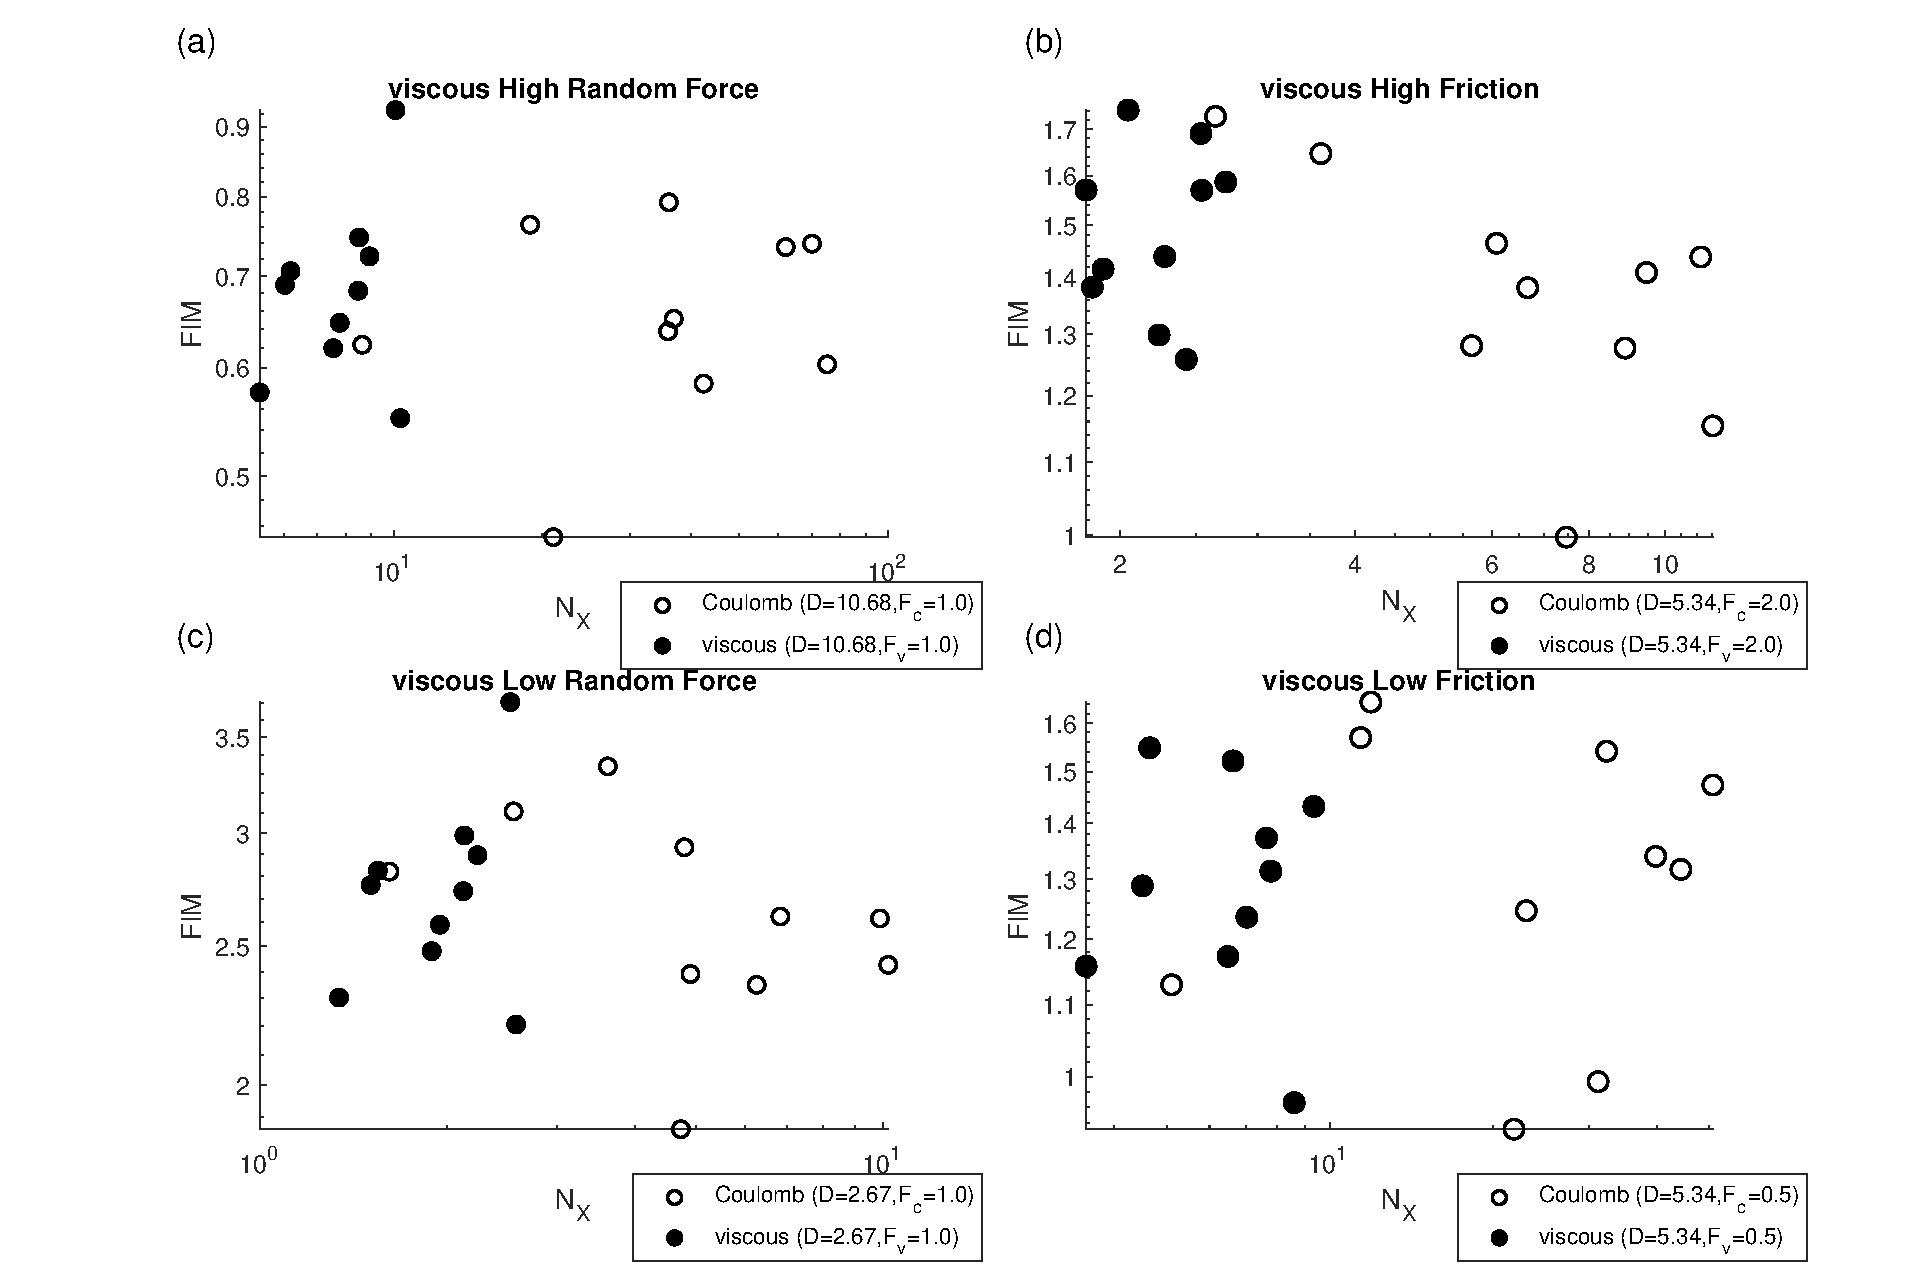
\includegraphics[width=\textwidth]{NEW-2b.eps}
    % 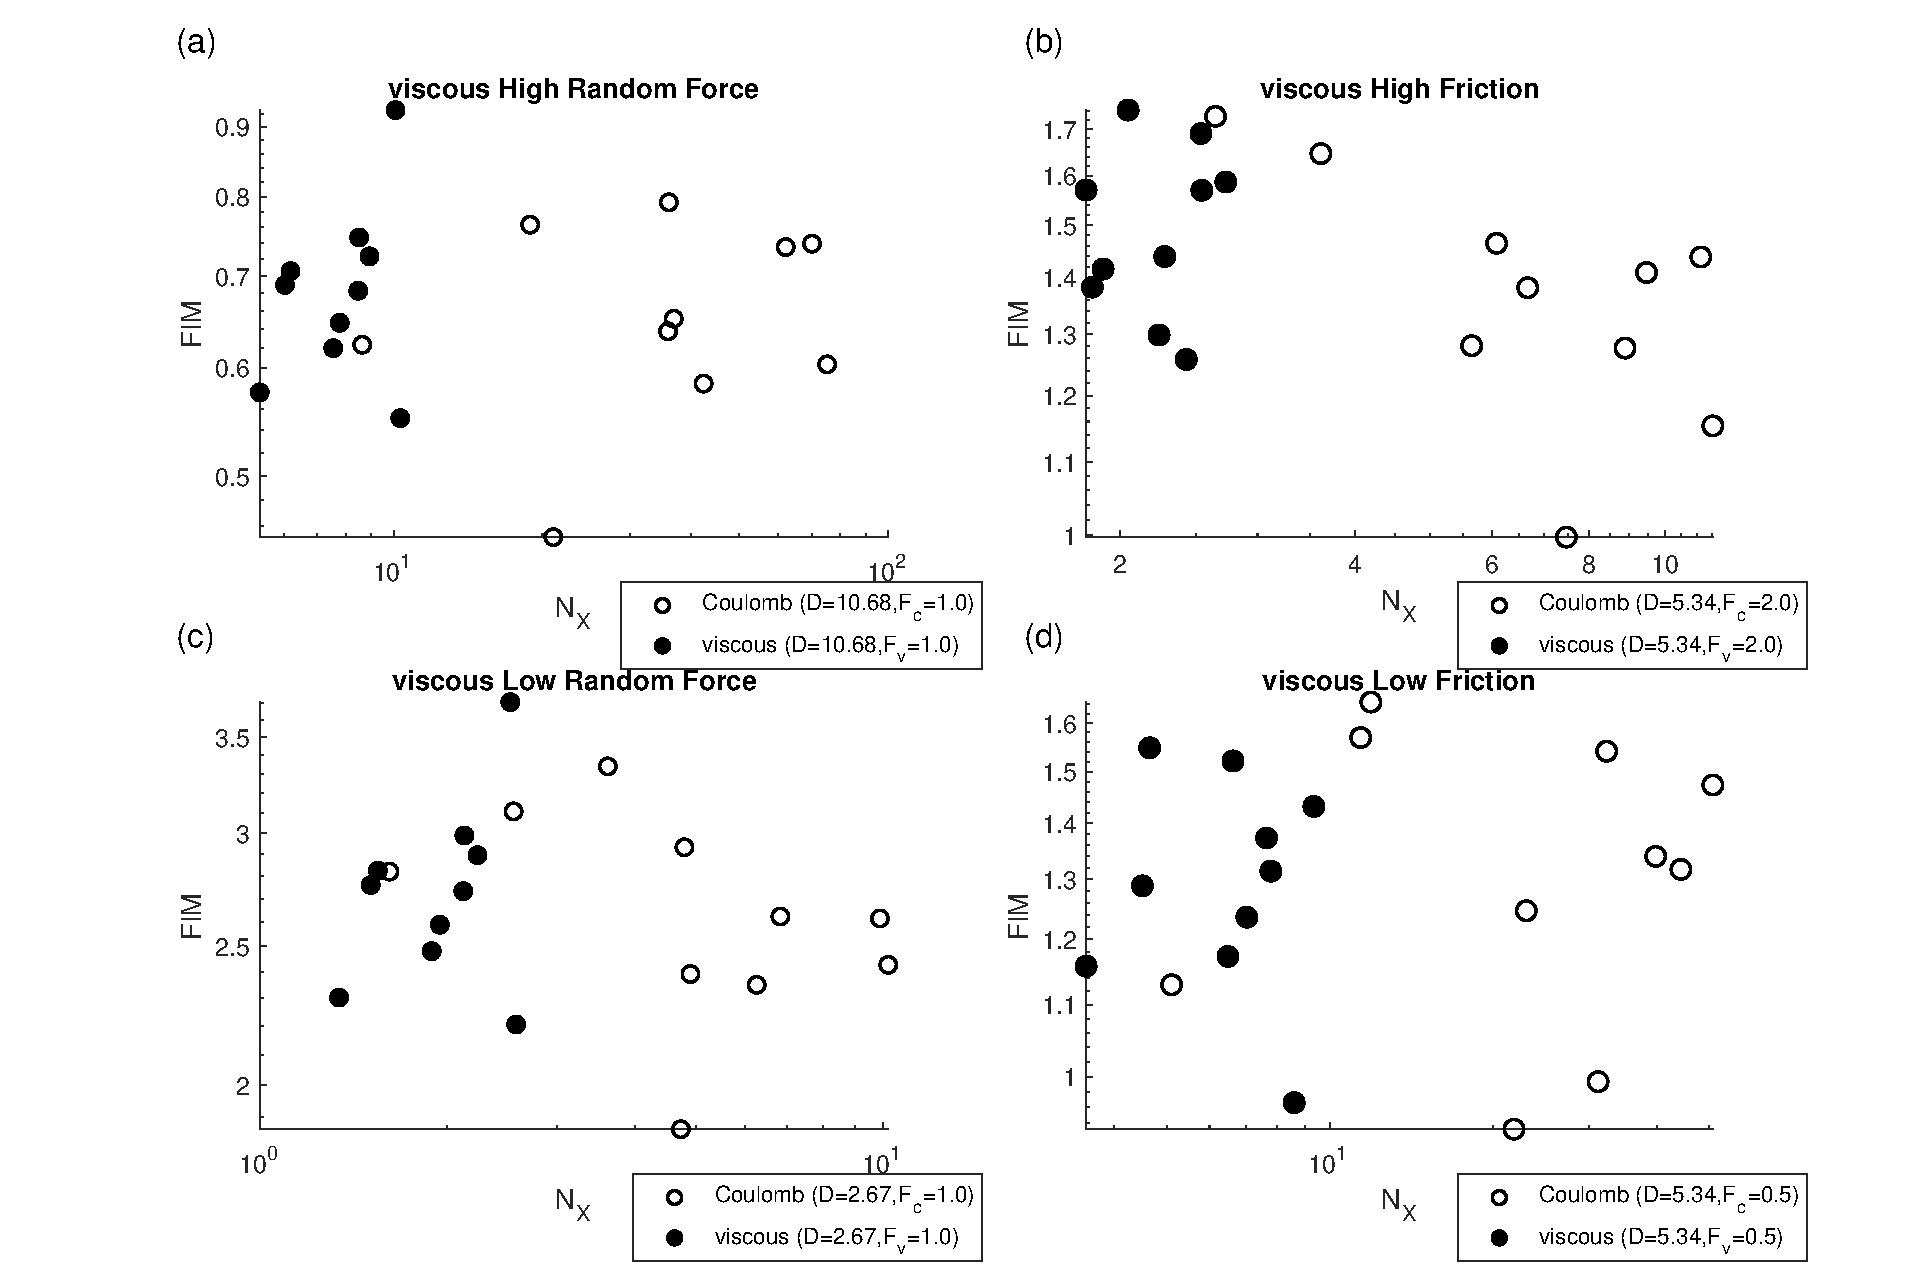
\includegraphics[width=0.5\textwidth]{NEW-2b.eps}
    \caption{\label{f_new}
        Four sets of time series generated with different levels of random force or friction are displayed on the FS-plane.
        There are 10 realizations in each sets; each realization has the same length (30 simulation time or $3\times 10^6$ points) as the original (non-window--averaged) ones in Fig. \ref{fig_smth}.
        The value of diffusion coefficient and friction parameter are described in the legend, while other parameters remain the same.
        %  as the original ones.
        %The friction parameter ($F_C$ or $F_v$) is 2 in the high friction set; 0.5 in the low friction set; other parameters remain the same as the original set.
        %The diffusion coefficient $D$ is 10.68 in the high random force set; 2.67 in the low random force set; other parameters remain the same as the original set.
        % The diffusion coefficients ($D$) in original, low- and high-friction sets are 5.34; the friction parameters in original, low and high random force sets are 1.
        % Among triangle markers, purple ones have the same value of friction parameter as the original ones, while magenta ones have the same value of diffusion coefficient $D$ as the original ones.
        % ; in the original set is 1. 
        % (The original set has friction parameter 1, and diffusion coefficient 5.34 as described previously.)
        % ($F_C$ for Coulombian and $F_v$ for viscous case)
    }
\end{figure*}

Concerning different level of friction and random force, four sets of synthetic time series under a higher/lower friction parameter and a higher/lower diffusion coefficient are generated respectively.
The result are displayed in Fig. \ref{f_new}.
In conditions of high (low) random force, the diffusion coefficient $D$ is twice (half) of that in the original set, while the friction parameter remains the same (Fig. \ref{f_new} a,c).
Similarly, in conditions of high (low) friction, the friction parameter $F_{c/v}$ is twice (half) of that in the original set, while the diffusion coefficient remains the same (Fig. \ref{f_new} b, d). The results show that the realizations under the high (low) level of random force as well as under high (low) friction show a FS pattern very similar to that shown in Fig. 3, where clearly the separation between the two frictional mechanisms is evidenced.


\section{Discussion and conclusion}
The obtained results point out to the following findings. The FS method allows to discriminate between two different frictional regimes that occur in earthquake rupture processes: viscous and Coulombian. In particular the lower Shannon entropy that emerged in the viscous frictional regime suggests that a more ordered and more organized status characterizes fault system.

The smaller Shannon entropy in viscous frictional regime seems to be reflected in the informational characteristics of the structure of the surfaces of the fault planes. Nosonovsky \cite{nosonovsky_entropy_2010}, investigating the relationship between friction and entropy, proposed the Shannon entropy as a parameter to describe the adjustment of sliding surfaces, and, practically, as a measure of the roughness of a surface. Therefore, surface profiles with smaller Shannon entropy are  more “ordered” (or less random) than those with a larger Shannon entropy. Thus, a smooth surface is characterized by the lowest possible value of the Shannon entropy, which is zero, while a random surface profile by a larger value. Recently, Moreno-Torres et al. \cite{moreno-torres_investigating_2018} have analysed the informational properties of the voltage measured during stick-slip experiments of a block sliding on the same rough surface for several consecutive runs; they found that the Shannon entropy of the stick-slip related voltage series decreases with the run, being the larger in the first run and the smallest in the last run. After each run, the asperities on the rough surface become lower making the surface smoother and smoother; the sliding, then, is facilitated as it would happen if the interface between the two rough surfaces is properly lubricated. Very probably, in the stick-slip experiments some dust is produced during each run that could fill the space between the asperities acting as a sort of lubricant, increasing the smoothing of the surfaces; such increase is reflected in the smaller Shannon entropy. Moreover, a higher FIM is observed with the increase of the smoothness of the surfaces in mutual contact.

The analogy between the results of Moreno-Torres et al.  \cite{moreno-torres_investigating_2018} and ours can be stated, because at low velocities, in a Coulombian frictional regime sliding is harder than in a viscous frictional regime; this situation can be considered analogous to the presence of asperities between the fault planes that hinder the sliding and lead to the increase of the Shannon entropy. On the other hand, after taking into account the effect of smoothing, our results present a higher FIM as the frictional mechanism changes from Coulomb to viscous regime, also consistent with the increase of FIM after consecutive runs in the block-sliding experiments \cite{moreno-torres_investigating_2018}.

%(highlight)
The performance of Fisher information and Shannon entropy in characterizing different sets of time series provides hints how friction and random force affect the rupture process in different time scales.
The result displayed in Fig. \ref{f_new} suggests that Shannon entropy increases with a larger random force, a smaller friction parameter, or a less lubricated surface.
On the other hand, the Fisher information decreases with a larger random force, and barely changes among different friction mechanisms or friction parameters.
% $N_X$ can clearly separate different friction mechanism. Furthermore, it reflects the level of friction.
%Mathematically, Shannon entropy is a global measure of smoothness in the probability density function $f(x)$ of the time series $x(t)$, while Fisher information is a local measure of that \cite{frieden_physics_1998}. 
Being a local measure of smoothness in the probability density function of the time series, Fisher information is sensitive to the random force which dominates the evolution of the process in the microscopic time scale, and is insensitive to friction because the effect of friction is rather chronic.
Being a global measure, Shannon entropy performs well in distinguishing different friction mechanisms, levels of friction and random force.
This implies that the average strength of the random force, friction level, and the type of friction mechanism all have profound contributions to the macroscopic (long-term) behavior of the stochastic friction process.

In this study, an oversimplification is made that both Langevin equations of Coulomb and viscous friction have the same random force $\Gamma (t)$, whereas in a realistic scenario, weaker and less frequent interactions between asperities are expected in a more lubricated friction process.
However, a more inactive $\Gamma (t)$ in the viscous regime will only lead to an even lower $N_X$ and a higher FIM, that such simplification does not negate the implications of this study.

More insights can be obtained from the proposed stochastic dynamics for friction processes. Earthquakes, which are manifestations of the chaotic interacting forces between asperities of two plates, are temporally microscopic phenomena in a long-term friction process driven by the tectonic motion.
For a friction process between two tectonic plates modelled by the Langevin equation, an earthquake is considered as a realization of this stochastic process, and its size depends on the following three factors.
The first one is the duration of an event, which is determined when the rupture as a Brownian walk exceeds a certain threshold, sustains for a significant time interval, and falls below the threshold again.
The second one is the damping coefficient ($F_v$ or $F_C$) that hinders dislocations.
They are mostly determined by the properties of the two surfaces, loading stress and the condition of lubrication as presented in many studies \cite{hess_friction_1990,brodsky_elastohydrodynamic_2001,armstrong-helouvry_control_1991,nosonovsky_entropy_2010}.
The third one is the diffusion coefficient $D$. It reflects the average strength level of the random fluctuating force that promotes microscopic dislocations, and hence is assumed to depend on pre-slip conditions.
If both damping and diffusion coefficients are known, the average slip velocity of the stochastic rupture process can be calculated\cite{wu_stochastic_2018}.
In summary, for a stochastic rupture process, a deterministic estimation of the average slip velocity is possible, while the duration is determined by chance.
Given a fixed rupture area, the magnitude of an event is therefore the time integral of the stochastic rupture process with a mostly deterministic average slip velocity over a stochastic length of time.
This gives a similar conclusion as the widely cited cascade model \cite{kilb_initial_1999,ellsworth_observation_1998,brune_implications_1979}, where the size of an earthquake cannot be determined until the end of the rupture.
In the meanwhile, the estimation of diffusion/damping coefficient in an early stage of an event could provide some information about the average dislocation, and this could be referred to the partially deterministic nature of an earthquake rupture process as reported\cite{olson_deterministic_2005,wu_magnitude_2006}.

By the results of the present work, it could be suggested the possibility to determine the dominating frictional mechanism of the earthquake source process, if there were a robust way of turning the earthquake source model (obtained from inversion of the recorded seismic wave) into a time series.
Furthermore, the Langevin physics of friction provides a new point of view to both the deterministic and stochastic natures of earthquake rupture, considering earthquakes as microscopic processes of friction occurring in macroscopic tectonic deformation.


\begin{acknowledgments}
    % We wish to acknowledge the support of the author community in using
    % REV\TeX{}, offering suggestions and encouragement, testing new versions,
    % \dots.
    This work was partially supported by Ministry of Science and Technology, Taiwan (MOST) through 106WGEFA0700007 and Consiglio Nazionale delle Ricerche (CNR), Italy.

\end{acknowledgments}

% \appendix

% \section{Appendixes}




\nocite{*}

\bibliography{Ref_1}% Produces the bibliography via BibTeX.

\end{document}
%
% ****** End of file aipsamp.tex ******


% @Article{wen_multiplefault_2018,
%   author  = {Wen, Yi‐Ying and Ma, Kuo‐Fong and Fry, Bill},
%   title   = {Multiple‐{Fault}, {Slow} {Rupture} of the 2016 {Mw} 7.8 {Kaikōura}, {New} {Zealand}, {Earthquake}: {Complementary} {Insights} from {Teleseismic} and {Geodetic} {DataMultiple}‐{Fault}, {Slow} {Rupture} of the 2016 {Kaikōura} {Earthquake}},
%   journal = {Bull. Seismol. Soc. Am.},
%   year    = {2018},
%   volume  = {108},
%   number  = {3B},
%   pages   = {1774--1783},
%   issn    = {0037-1106},
% }

% @Article{siriki_laboratory_2015,
%   author  = {Siriki, Hemanth and Bhat, Harsha S and Lu, Xiao and Krishnan, Swaminathan},
%   title   = {A {Laboratory} {Earthquake}‐{Based} {Stochastic} {Seismic} {Source} {Generation} {Algorithm} for {Strike}‐{Slip} {Faults} and its {Application} to the {Southern} {San} {Andreas} {Fault}},
%   journal = {Bull Seismol Soc Am},
%   year    = {2015},
%   volume  = {105},
%   number  = {4},
%   pages   = {2250--2273},
%   issn    = {0037-1106},
%   doi     = {10.1785/0120140110},
% }

% @book{meyers_extreme_2011,
% 	address = {New York, NY},
% 	title = {Extreme {Environmental} {Events}},
% 	isbn = {978-1-4419-7694-9 978-1-4419-7695-6},
% 	url = {http://link.springer.com/10.1007/978-1-4419-7695-6},
% 	language = {english},
% 	urldate = {2018-02-22},
% 	publisher = {Springer New York},
% 	editor = {Meyers, Robert A.},
% 	year = {2011},
% 	doi = {10.1007/978-1-4419-7695-6}
% }